\documentclass[tikz,border=7pt]{standalone}
\usepackage[T1]{fontenc}
\usepackage{lmodern}
\usepackage{helvet}
\renewcommand{\familydefault}{\sfdefault}
\usepackage{amsmath}
\usepackage{xcolor}
\usepackage{tikz}
\usetikzlibrary{
  arrows.meta,
  positioning,
  calc,
  fit,
  shapes.geometric,
  shapes.symbols,
  backgrounds,
  decorations.pathreplacing,
  decorations.pathmorphing,
}

\definecolor{slate}{HTML}{334155}
\definecolor{teal}{HTML}{0D9488}
\definecolor{amber}{HTML}{D97706}
\definecolor{rose}{HTML}{E11D48}
\definecolor{muted}{HTML}{64748B}
\definecolor{line}{HTML}{94A3B8}
\definecolor{pagebg}{HTML}{F8FAFC}
\definecolor{card}{HTML}{FFFFFF}
\definecolor{lightteal}{HTML}{CCFBF1}
\definecolor{lightamber}{HTML}{FEF3C7}
\definecolor{lightrose}{HTML}{FFE4E6}
\definecolor{lightslate}{HTML}{E2E8F0}
\definecolor{blueink}{HTML}{2563EB}
\definecolor{bluewash}{HTML}{DBEAFE}
\definecolor{greenink}{HTML}{16A34A}
\definecolor{greenwash}{HTML}{DCFCE7}
\definecolor{pinkink}{HTML}{DB2777}
\definecolor{pinkwash}{HTML}{FCE7F3}

\tikzset{
  >=Stealth,
  font=\sffamily\scriptsize,
  every node/.append style={text=slate},
  title/.style={font=\sffamily\bfseries\small, text=slate, anchor=west},
  note/.style={font=\sffamily\tiny, text=muted, align=left},
  label/.style={font=\sffamily\tiny, text=muted},
  chip/.style={
    draw=#1,
    fill=#1!12,
    rounded corners=2pt,
    inner sep=2.5pt,
    font=\sffamily\tiny\bfseries,
    text=slate,
  },
  decision/.style={
    shape=diamond,
    aspect=2.1,
    draw=teal,
    fill=lightteal,
    inner sep=1.5pt,
    align=center,
    font=\sffamily\tiny,
    text=slate,
  },
  pics/person/.style 2 args={
    code={
      \fill[#1] (0,0.92) circle (0.18);
      \fill[#1]
        (-0.26,0.68)
        .. controls (-0.34,0.42) and (-0.30,0.18) .. (-0.22,0.02)
        -- (0.22,0.02)
        .. controls (0.30,0.18) and (0.34,0.42) .. (0.26,0.68)
        -- cycle;
      \node[font=\sffamily\tiny\bfseries, text=#1, anchor=north] at (0,-0.08) {#2};
    }
  },
  pics/disk/.style={
    code={
      \fill[lightslate] (0,-0.04) ellipse (0.28 and 0.10);
      \fill[slate] (-0.28,-0.04) rectangle (0.28,0.12);
      \fill[slate] (0,0.12) ellipse (0.28 and 0.10);
      \fill[card] (0,0.14) ellipse (0.11 and 0.04);
    }
  },
}

\begin{document}
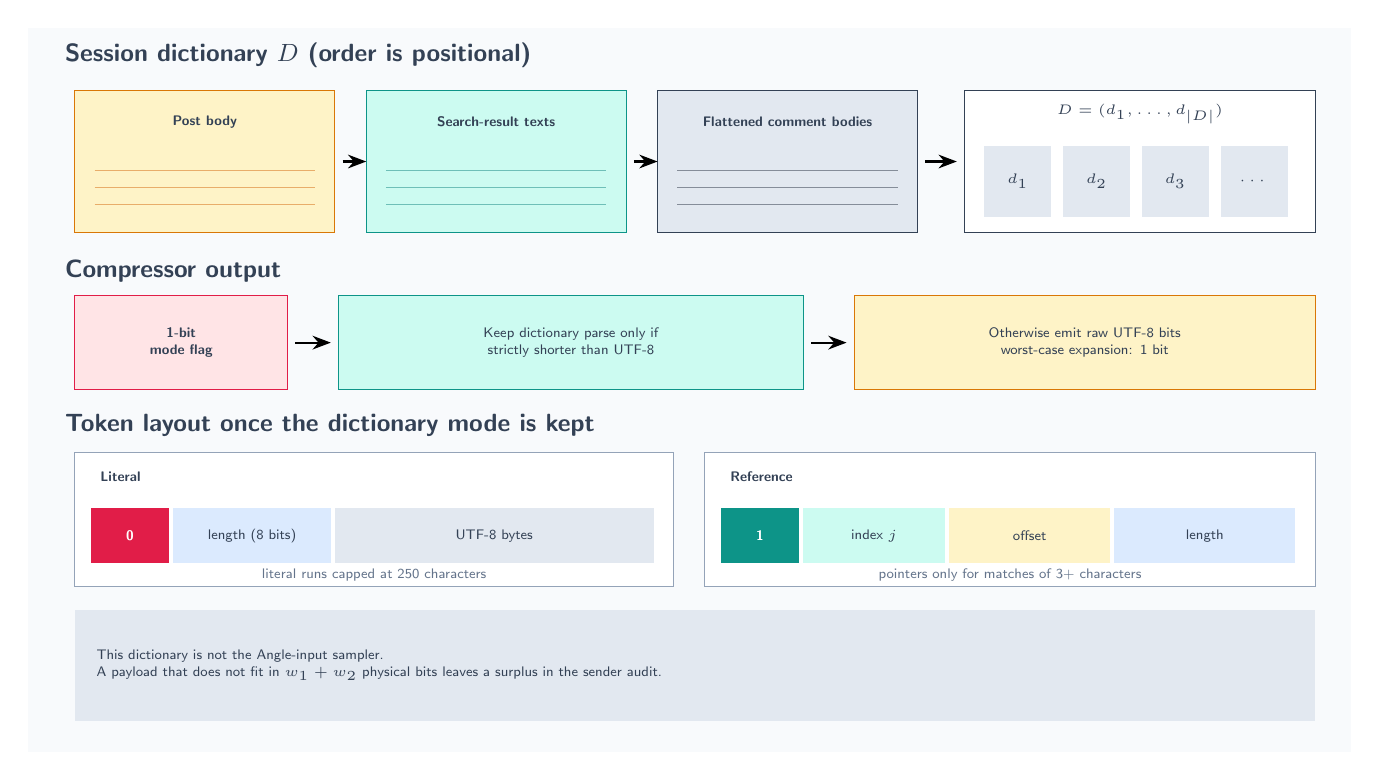
\begin{tikzpicture}[x=1cm,y=1cm]
  \fill[pagebg] (-0.3,-0.25) rectangle (16.5,8.95);
  \node[title] at (0.05,8.60) {Session dictionary $D$  (order is positional)};

  % three source stacks merging
  \foreach \x/\fillc/\drawc/\lab in {
    0.3/lightamber/amber/Post body,
    4.0/lightteal/teal/Search-result texts,
    7.7/lightslate/slate/Flattened comment bodies} {
    \fill[\fillc] (\x,6.35) rectangle (\x+3.3,8.15);
    \draw[\drawc] (\x,6.35) rectangle (\x+3.3,8.15);
    \foreach \dy in {0.0,0.22,0.44} {
      \draw[\drawc!60] (\x+0.25,6.70+\dy) -- (\x+3.05,6.70+\dy);
    }
    \node[font=\sffamily\tiny\bfseries] at (\x+1.65,7.75) {\lab};
  }
  \draw[thick, ->] (3.7,7.25) -- (4.0,7.25);
  \draw[thick, ->] (7.4,7.25) -- (7.7,7.25);
  \draw[thick, ->] (11.1,7.25) -- (11.5,7.25);

  % D shelf
  \fill[card] (11.6,6.35) rectangle (16.05,8.15);
  \draw[slate] (11.6,6.35) rectangle (16.05,8.15);
  \node[font=\sffamily\tiny\bfseries] at (13.825,7.85) {$D=(d_1,\ldots,d_{|D|})$};
  \foreach \i/\lab in {0/$d_1$, 1/$d_2$, 2/$d_3$, 3/$\cdots$} {
    \fill[lightslate] (11.85+1.0*\i,6.55) rectangle (12.70+1.0*\i,7.45);
    \node[font=\sffamily\tiny] at (12.275+1.0*\i,7.00) {\lab};
  }

  \node[title] at (0.05,5.85) {Compressor output};
  \fill[lightrose] (0.3,4.35) rectangle (3.0,5.55);
  \draw[rose] (0.3,4.35) rectangle (3.0,5.55);
  \node[font=\sffamily\tiny\bfseries, align=center] at (1.65,4.95) {1-bit\\mode flag};
  \draw[thick, ->] (3.1,4.95) -- (3.55,4.95);

  \fill[lightteal] (3.65,4.35) rectangle (9.55,5.55);
  \draw[teal] (3.65,4.35) rectangle (9.55,5.55);
  \node[font=\sffamily\tiny, align=center, text width=5.5cm] at (6.6,4.95) {Keep dictionary parse only if\\strictly shorter than UTF-8};

  \draw[thick, ->] (9.65,4.95) -- (10.10,4.95);

  \fill[lightamber] (10.20,4.35) rectangle (16.05,5.55);
  \draw[amber] (10.20,4.35) rectangle (16.05,5.55);
  \node[font=\sffamily\tiny, align=center, text width=5.5cm] at (13.125,4.95) {Otherwise emit raw UTF-8 bits\\worst-case expansion: 1 bit};

  \node[title] at (0.05,3.90) {Token layout once the dictionary mode is kept};

  % literal anatomy
  \fill[card] (0.3,1.85) rectangle (7.9,3.55);
  \draw[line] (0.3,1.85) rectangle (7.9,3.55);
  \node[font=\sffamily\tiny\bfseries, anchor=west] at (0.5,3.25) {Literal};
  \fill[rose] (0.5,2.15) rectangle (1.5,2.85);
  \node[font=\sffamily\tiny\bfseries, text=card] at (1.0,2.50) {0};
  \fill[bluewash] (1.55,2.15) rectangle (3.55,2.85);
  \node[font=\sffamily\tiny] at (2.55,2.50) {length (8 bits)};
  \fill[lightslate] (3.60,2.15) rectangle (7.65,2.85);
  \node[font=\sffamily\tiny] at (5.625,2.50) {UTF-8 bytes};
  \node[note] at (4.1,2.00) {literal runs capped at 250 characters};

  % reference anatomy
  \fill[card] (8.3,1.85) rectangle (16.05,3.55);
  \draw[line] (8.3,1.85) rectangle (16.05,3.55);
  \node[font=\sffamily\tiny\bfseries, anchor=west] at (8.5,3.25) {Reference};
  \fill[teal] (8.5,2.15) rectangle (9.5,2.85);
  \node[font=\sffamily\tiny\bfseries, text=card] at (9.0,2.50) {1};
  \fill[lightteal] (9.55,2.15) rectangle (11.35,2.85);
  \node[font=\sffamily\tiny] at (10.45,2.50) {index $j$};
  \fill[lightamber] (11.40,2.15) rectangle (13.45,2.85);
  \node[font=\sffamily\tiny] at (12.425,2.50) {offset};
  \fill[bluewash] (13.50,2.15) rectangle (15.80,2.85);
  \node[font=\sffamily\tiny] at (14.65,2.50) {length};
  \node[note] at (12.175,2.00) {pointers only for matches of 3+ characters};

  \fill[lightslate] (0.3,0.15) rectangle (16.05,1.55);
  \node[font=\sffamily\tiny, text width=15.2cm, align=left] at (8.175,0.85) {%
    This dictionary is not the Angle-input sampler.\\
    A payload that does not fit in $w_1+w_2$ physical bits leaves a surplus in the sender audit.};
\end{tikzpicture}
\end{document}
